%Architecture
In this section we describe in detail the system architecture, in particular the memory hierarchies along with the data mapping and refresh policies that we adopt.

\begin{figure*}[ht!]
\begin{minipage}[b]{0.36\linewidth}
\raggedleft
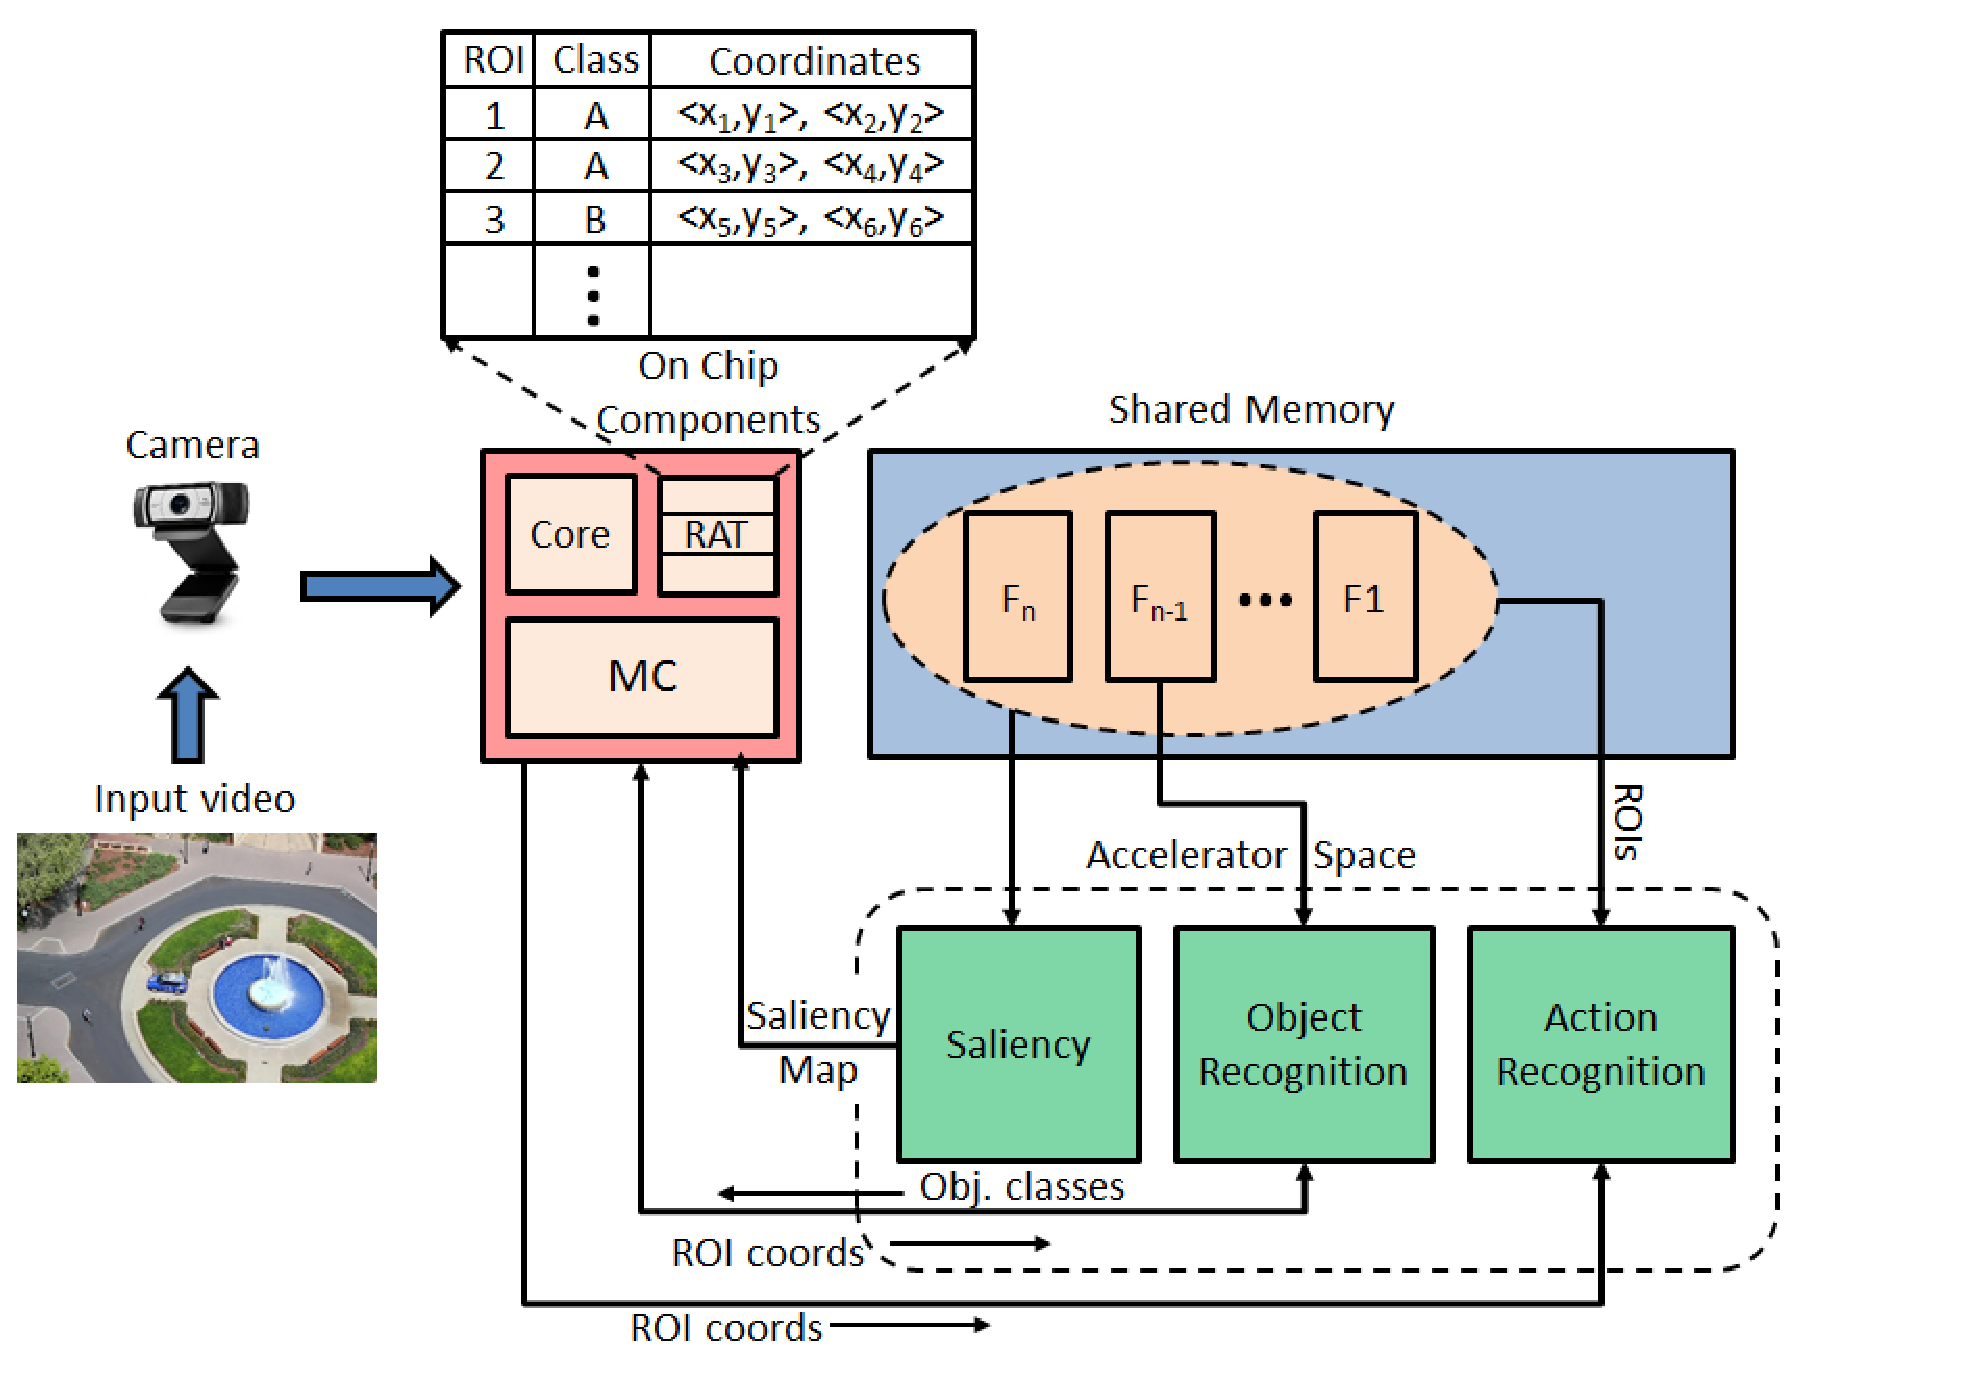
\epsfig{file=figs/baseline_arch.eps, angle=0, width=1\linewidth, clip=}
\caption{\label{fig:reva}a) Baseline architecture}
\end{minipage}
\addtocounter{figure}{-1}
\begin{minipage}[b]{0.37\linewidth}
\centering
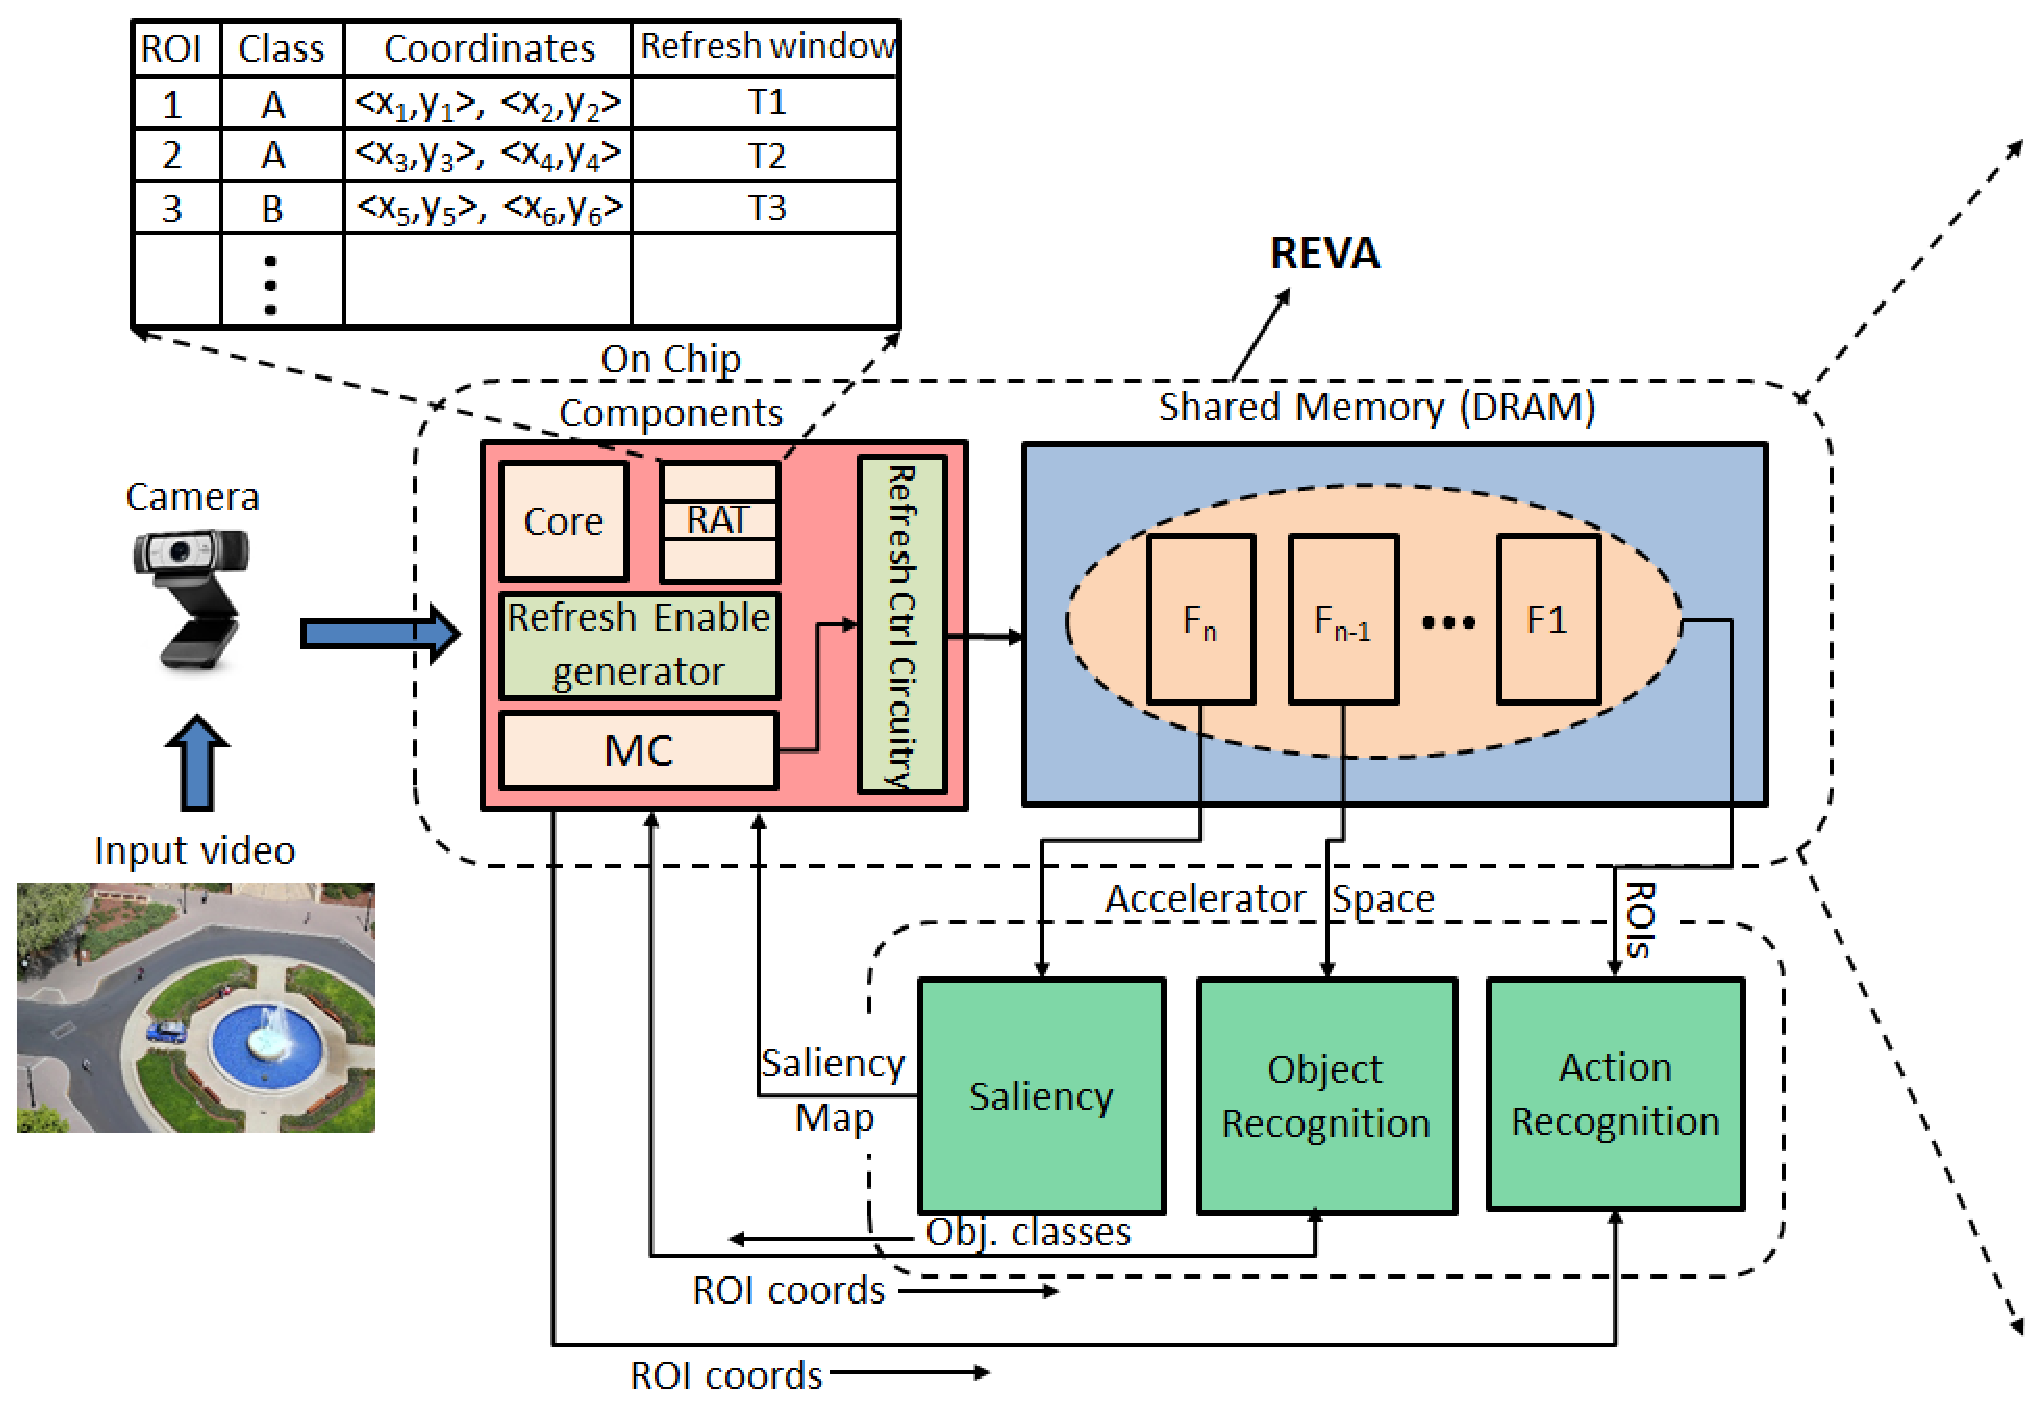
\epsfig{file=figs/reva_arch.eps, angle=0, width=1\linewidth, clip=}
\caption{\label{fig:reva}b) Architecture of Proposed System}
\end{minipage}
\addtocounter{figure}{-1}
\begin{minipage}[b]{0.25\linewidth}
\raggedright
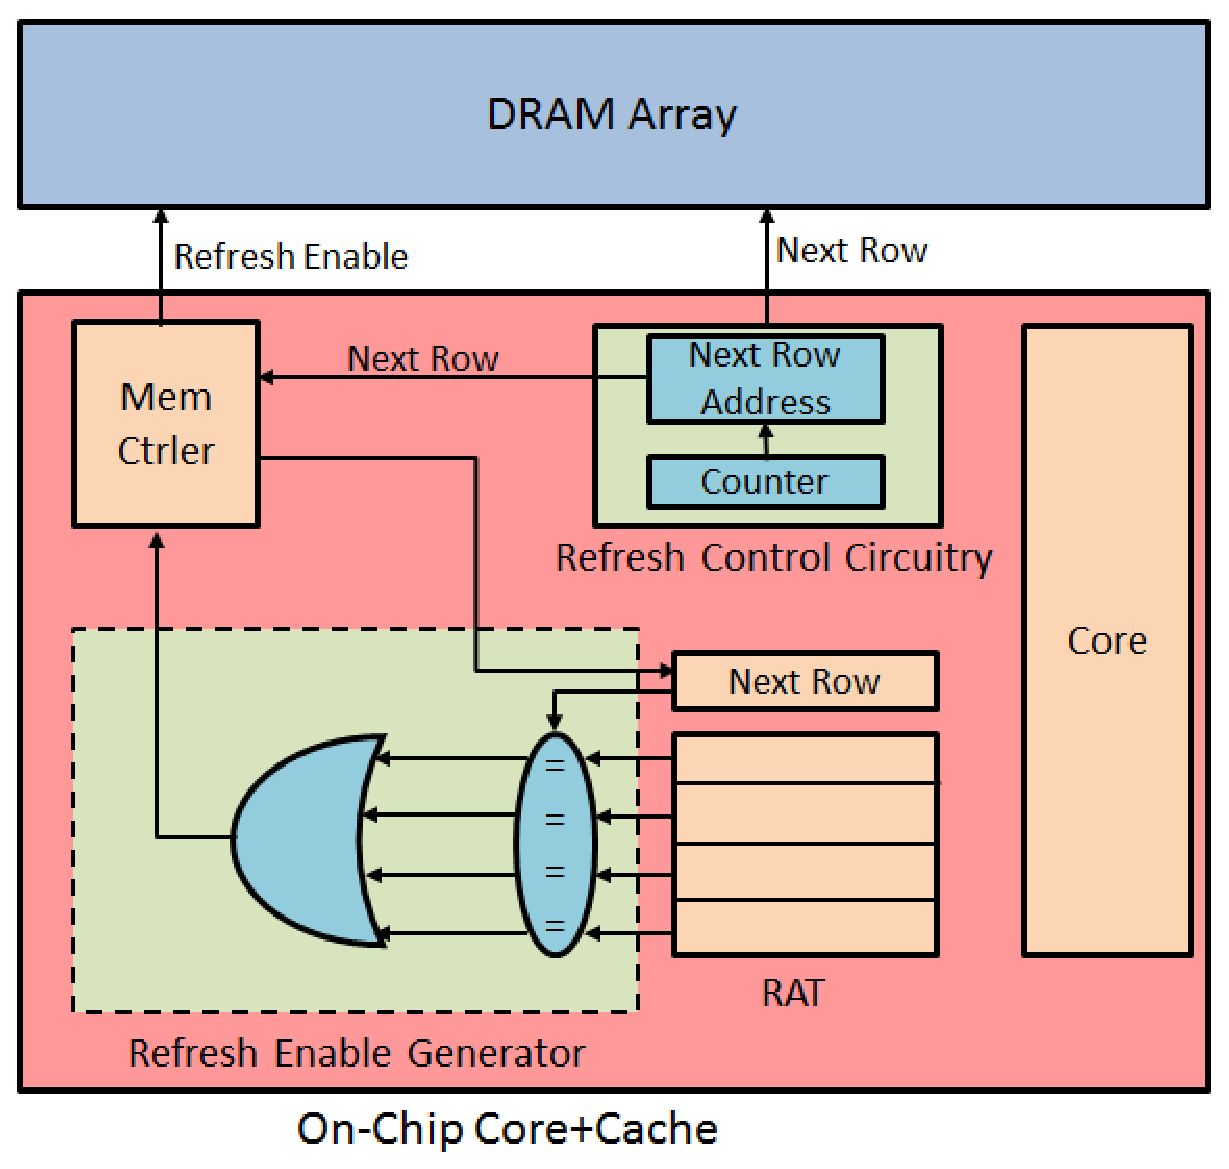
\epsfig{file=figs/refresh_circuitry.eps, angle=0, width=1\linewidth, clip=}
\caption{\label{fig:reva}c) Design of REVA block}
\end{minipage}
\end{figure*}


Figure~\ref{fig:reva}a) illustrates the baseline architecture for the vision analytics-based system. The input video is captured by the HD camera at a rate of 30 frames/s. 
These frames are stored in the off-chip DRAM, as shown in the figure. These frames are then read by the saliency accelerator is used to compute a \emph{Saliency Map}. This saliency map is then used to compute the RoIs by the CPU, which are then stored on-chip in a table known as the \emph{RoI Address Table (RAT)}. Each entry in the table corresponds to an RoI, and has a list of coordinates that specify its position in each frame. 
The Object Recognition accelerator classifies the objects in each ROI as belonging to a certain class. This information is also appended in the RAT.
On the other hand, the Action Recognition Engine requires a series of consecutive frames to classify the exact action being carried out. 
Since each of these frames over the entire length of the video stored in the main memory module, there is a substantial overhead, especially in terms of refresh energy, in the baseline architecture. 

In our proposed design, shown in Figure~\ref{fig:reva}b), we recognize that the DRAM primarily serves the purpose of a stream buffer. Consequently the frames are rarely reused after processing, which may eliminate the need for refresh entirely. 
However, some accelerator operations, especially action recognition, which occurs on certain objects require a sequence of previously stored frames to be recalled. Hence, we only need to \emph{selectively} refresh the RoIs involved in these functions. We thus propose differential refresh rates based on the RoI and object class with which it has been associated by the object recognition engine.
We thus use a scheme called \emph{Differential Refresh}, shown in Figure~\ref{fig:reva}c), for which we describe the setup below.

\subsection{Differential Refresh Architecture}
As explained above, in the time duration of Refresh Cycle Time ($T_{RFC}$), a group of rows is refreshed sequentially when a refresh pulse is scheduled. A refresh pulse is sent every Refresh Interval ($T_{ref}$) time period.  When a refresh is scheduled, we keep track of the next row to be refreshed in a bank in the Next\_Row\_Address register. At the end of every refresh iteration, the content of this register is sent to the memory controller. At the memory controller, we maintain a CAM structure, RoI Address Table (RAT) to list Regions of Interest in each frame and their corresponding starting addresses. When the address of the next row to be refreshed does not match an RoI address on associative search, Refresh Enable signal is set to 0. This ensures that rows of an image in a bank that do not belong to RoIs are refreshed less frequently than the rows that contain Regions of Interest. We propose two schemes to support differential Refresh rates across different sections of an image. 

Each image frame is interleaved across banks at page granularity utilizing Row Buffer Locality. The saliency accelerator computes RoIs and updates the RAT~\ref{fig:reva}c) which is forwarded to the memory controller. After a refresh iteration, when the memory controller gets the Next\_Row\_Address and a match for this is found in the RAT, a refresh pulse is sent to the command queue; otherwise Refresh Enable signal is set to low. An RoI is a 2-d rectangular tile and might correspond to different rows in different banks; the group of rows containing a portion of the RoI might also have non-RoI regions striped across multiple banks. Still, the energy overhead of refreshing non-RoI regions in rows that contain RoI is x\% lesser than the energy overhead incurred on applying a uniform auto-refresh policy to the entire image. Since the non-RoI regions of the image are not subsequently read/written to, we allow the non-critical sections of the image to degrade with infrequent refreshes.  

It needs to be noted that for completely stream-based processing, where there is a single-pass streaming access of the image, a no-refresh policy can be implemented for the entire image allowing corruption. Since a read operation inherently involves a refresh and each image row is read no more than once, this results in a no-refresh policy. 

This scheme involves communication overhead between memory controller and the refresh controller since the address of the next row to be refreshed is sent after every refresh iteration. An alternative would be to assign fixed refresh rates for different sections of a bank. For example, the upper addresses of a bank can be configured for no refresh and the lower addresses for auto-refresh policy. However this would involve mapping the physical pages of a Region of Interest to a specific partition in the bank incurring additional OS overhead and the scheme we propose does not involve page-level mapping of Virtual Addresses of RoIs to physical pages of a partition. Also, when the saliency accelerator generates the saliency map, RoIs are not written to dedicated variable refresh frequency partitions again. Instead the saliency map computed is used to derive RoIs in input image already stored in memory and refresh frequencies are varied based on the location of RoIs. 

\subsection{Comparison with existing schemes}
Selectively refreshing the DRAM depending on data criticality has been demonstrated earlier in~\cite{Liu2011}. However, unlike their scheme which consists of a static partitioning of the memory depending on the required refresh rate, our system is capable of dynamically allocating refresh periods to stripes of rows across banks. Consequently, by interleaving data across all banks, it is possible to control the refresh rates of each individual RoI. 

Figure~\ref{fig:reva-refresh} contrasts the two schemes described above.

\begin{figure}[ht!]
\centering
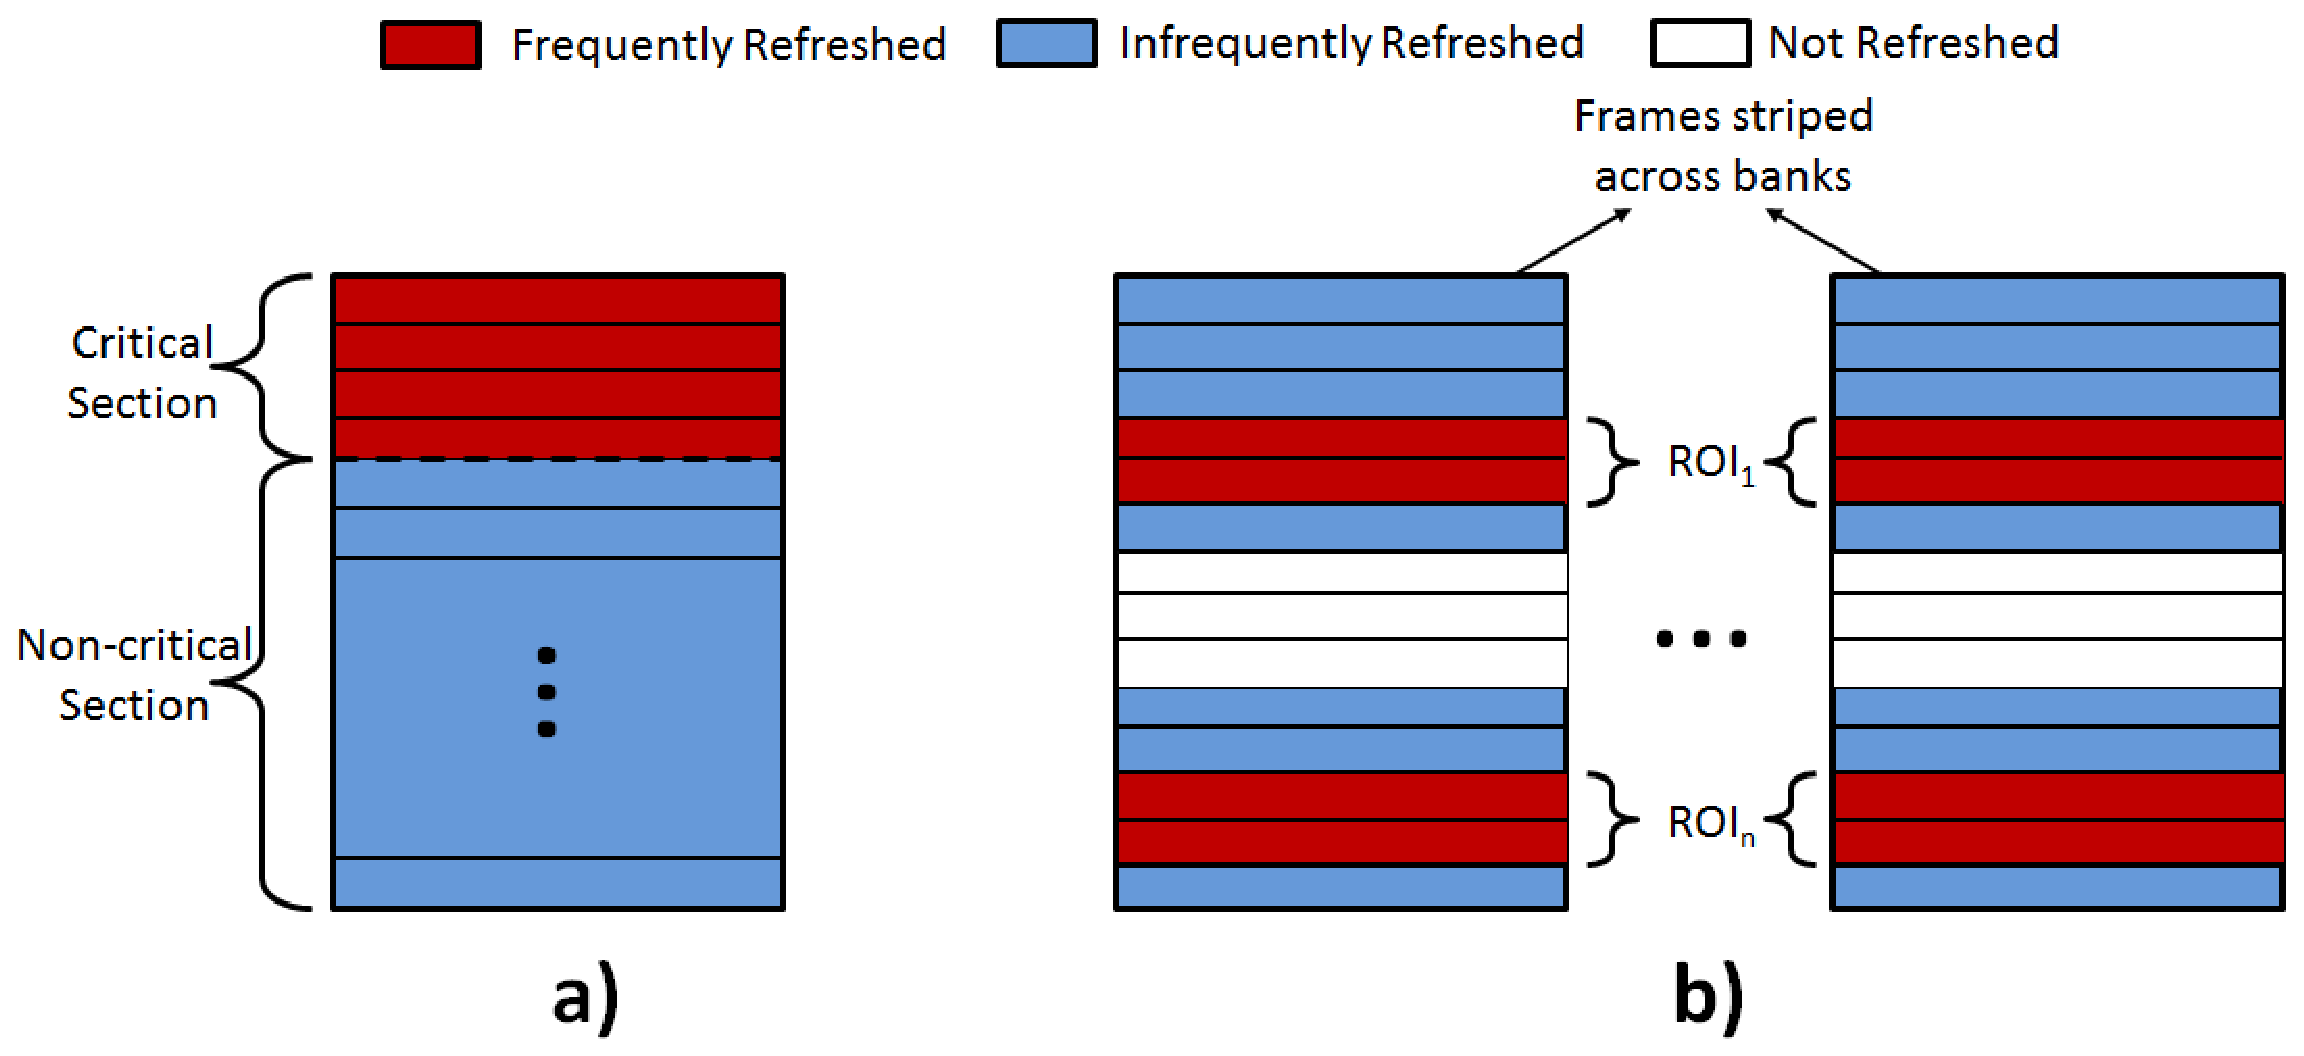
\epsfig{file=figs/reva_refresh.eps, angle=0, width=0.9\linewidth, clip=}
\caption{\label{fig:reva-refresh} }
\end{figure}
